\documentclass[12pt,a4paper]{article}
\usepackage[utf8]{inputenc}
\usepackage[english]{babel}
\usepackage{amsmath}
\usepackage{amsfonts}
\usepackage{amssymb}
\usepackage{graphicx}
\usepackage{subfig}
\usepackage{float}
\usepackage{listings}




\begin{document}
\title{\bf Financial Practicum Project }
\author{Andraž Pirnovar, Jaša Štefan, Laura Carvajal  \\ University of Ljubljana}
\date{November, 15th of 2017}
\maketitle{}
\begin{center}
{\small{\bf Summary}}\end{center}
\begin{quote}
{\small 
\ \ \ \ \ This project presents the numerical results of a problem related to the field of Operations Research. For the resolution of it, we have worked with the programming languages: \textit{Python, R} and \textit{Matlab}. You can find some graphs and tables in addition to a clear description of the problem and the main ideas of the program that we have used.}
\end{quote}
\bigskip 
\section{Problem description and objective}
Let us consider an annulus $A$. An annulus is a ring-shaped object, bounded by two concentric circles $C$ and $C'$. Let us assume that $C'$ is the smaller one. Inside the annulus, there is a set of n points, named $P_n$, that are uniformly randomly distributed. For these points, we find a convex hull $CH(P_n)$. A convex hull of a set of points $X$ in a Euclidean space (or affine space over the reals) is the smaller convex set that contains $X$. If we were to have a bounded set $X$ of points on a plane, we could visualise the convex hull as a rubber band stretched around the set $X$. \medskip 
 
The objective of our assignment is to experimentally analyse the length and the area of $CH(P_n)$. We also have to experimentally analyse the probability that the convex hull $CH(P_n)$ contains the inner border (smaller circumference) of the annulus, $C'$. 
\pagebreak 

\section{Hypothesis}
The results should depend on the proportion between the smaller and the bigger circle and also on the number of points inside the annulus.\medskip  
 
Our hypothesis is that the length of the convex hull will increase significantly with the number of points till a certain point and then only marginally with further increase. The size of the radius $r$ will also be a significant factor in the length of the hull, presumably even more so than $n$, as generated points will be squeezed to the outskirts of the annulus with the radius increase. Similar applies to the area.  \medskip 
 
The probability of the convex hull including the smaller circle, $C’$, should increase with $n$ and decrease with $r$. \medskip 
 
The method of point generation should be of some importance. Presumably, if points are generated \textit{“truly” uniformly}, the probability of inclusion should be higher than with the \textit{naive polar method}, as there will be more points on the outskirts of the annulus. Therefore, the convex hull from the “true” uniform distribution should be longer and should cover a larger area. Because of a bigger hull, we expect the probability of a smaller circle inclusion to be higher.
 
\section{Theoretical framework}
For the computing of the convex hull, we use two different convex hull generating methods. \textit{Quickhull} algorithm is used in the data generating algorithm and \textit{Gift Wrapping}, otherwise known as \textit{Jarvis March},  algorithm is used in the graph generating part. The Quickhull algorithm is called from the \textit{scipy} \textit{python} package, which uses the \textit{Qhull} library. We decided for this algorithm because it was already implemented in \textit{C++}, which means significant speed gains. The Gift Wrapping algorithm was implemented in \textit{python}, as  it is only used for drawing.

\subsection{Quickhull}

Quickhull algorithm uses a divide and conquer approach, similar to that of Quicksort. \\

The idea of the algorithm is:
\begin{enumerate}
	\item Find the points with the minimum and maximum $x$ coordinates, as they will always be a part of the convex hull.
	\item Use the line formed by connecting the two points to divide the points in two sets subsets of points, which will be 		processed recursively.
	\item Determine the point, farthest away from the line and form a triangle with it and the dividing line.
	\item Points inside the triangle can not be part of the convex hull, therefore they can be ignored.
	\item Repeat step \text{3.} and \text{4.} on the new lines, formed by the triangle.
	\item Repeat until no free points are left. The ones connected by the line (saved during execution of the algorithm)
	constitute the convex hull.
\end{enumerate}

The average time complexity is $O(n\log{n})$ and in worst possible case, $O(n^2)$

\subsection{Gift wrapping}

The first phase of the algorithm is to identify the minimum point on some axis. The $ y-axis $ is a good candidate, as the angles for all other points in the set range from $90^{\circ}$  to $270^ {\circ}$ , which facilitates sorting. This makes identifying the point with the minimum angle, relative to the current point, significantly easier.Starting with the minimal point, already known to be in the final perimeter, the algorithm scans all the points in the set, computes their angle, and stores the most angularly minimal point. Because the initial order of the set is arbitrary, it is necessary to scan all nodes in the set except for the current point. Sorting by angle is not useful, because the angles change as the algorithm progresses from point to point. The point found from the process described above will be the next point in the convex hull, in the clockwise direction. If you relate this to the physical example using the rubber band stretched around the set X it is evident that as you put the rubber around the set, the first pin that touches the string will be the one with the least relative angle.\medskip

The time complexity of this algorithm is $O(nh)$, where $n$ is the number of vertices, and $h$ is the number of vertices on the convex hull. This complexity is favourable where $n$ is small or $h$ is expected to be small, compared to $n$. \medskip

\section{Methodology}
Most of the programming work has been done in Python and Matlab, with some graphics and analysis done in R. Most of the project specific code was written by us, with the help of \textit{numpy} and \textit{scipy} packages.
\medskip

We created a new class called \textit{annulus}, in which most of the generating and computing functions were defined. Our class, methods and functions are called from the \textit{Script.py} file, in which we set the parameters for the data generation. More detailed description of our code is in the comments in the code itself. \medskip

The data was generated twice, using different values for $n$, once for analytical purposes and once for 3D plotting. The main analysis was done on the following set for $n$:
$$n= 3,4,5,6,7,8,9,10,15,20,30,40,50,100,200,500$$
We use two methods for point generation:
\begin{enumerate}
 \item The first one distributes the points uniformly over the area of the annulus, using a probability transformation of uniformly distributed polar coordinates.
 \item The other also uses uniformly distributed parameters of polar coordinates, but without the transformation, so the points are not uniformly distributed over the annulus, but are more common when $r$ is lower.
 \end{enumerate} 

%As is known, wee need to experimentally analyse the length, the area of CH(Pn), and also the probability that the convex hull CH(Pn) contains the inner border.
%At smaller values, the differences in length, area and probability should be more noticeable with small increases in n than at higher.\medskip

As we have to analyse the data with respect to radius $r$ of the smaller circle $C’$ and number of points $n$, we decided it would be best if we measure the radius relatively to the radius of the bigger circle.

So we set the bigger radius to $1$ and took $101$ smaller radiuses, from $0\to 1$. This represents $1\%$ increase of the smaller radius, relative to the bigger one, for which we calculate all of the required properties. \medskip

\begin{figure}[H]
 \centering
  {
   \label{f:graph1}
    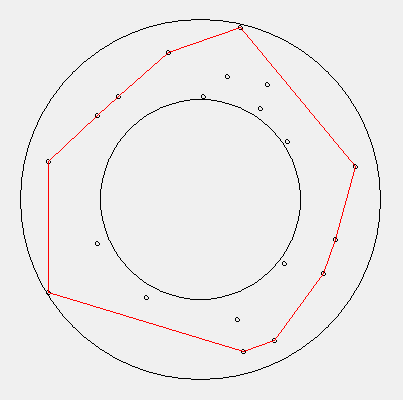
\includegraphics[width=0.3 \textwidth]{../graphs/convex_hull1.png}} \hspace{25mm}
  {
   \label{f:graph2}
    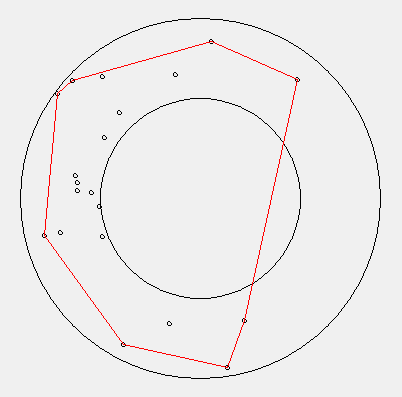
\includegraphics[width=0.3  \textwidth]{../graphs/convex_hull2.png}}
 \caption{Example of how the convex hull looks. In this case the set have 20 points.}
 \label{f:graphs}
\end{figure}

For each combination of $r$, $n$ and generating method, we did $4000$ repetitions, each time with a new set of randomly generated points. For every combination, we calculated \textit{mean length}, \textit{mean area} and the number of times the smaller circle $C’$ was included inside the convex hull. From this, we calculated the experimental probability of the convex hull containing the inner circle $C'$. \medskip
 
Data was saved to a \text{csv}, so that it was easy to import into \text{R} and make graphs to better show and compare the results.

\subsection{Time complexity of the generating algorithm (annulus class)}
The most demanding tasks are finding the convex hull, which is, at it's worst, $O(n^2)$, and figuring out, whether $C'$ is included inside the hull or not. This task is $O(h)$, where $h$ is the number of vertices on the convex hull, as distance calculation is constant to the input (points), and we calculate the distance $h$-times. Calculating the length takes $O(h)$ operations, as does calculating the area. As vertices are generated randomly, their generation has no standard time complexity, but we can say is, in worst case as there is $n$ random numbers, $O(n)$. This means that the time complexity for this algorithm is $O(n^2)$.

\section{Results}

We present the results through graphs made with R. 
\subsection{Length of the convex hull}

\begin{figure}[H]
 \centering
  \subfloat[With naive distribution]{
   \label{f:length1}
    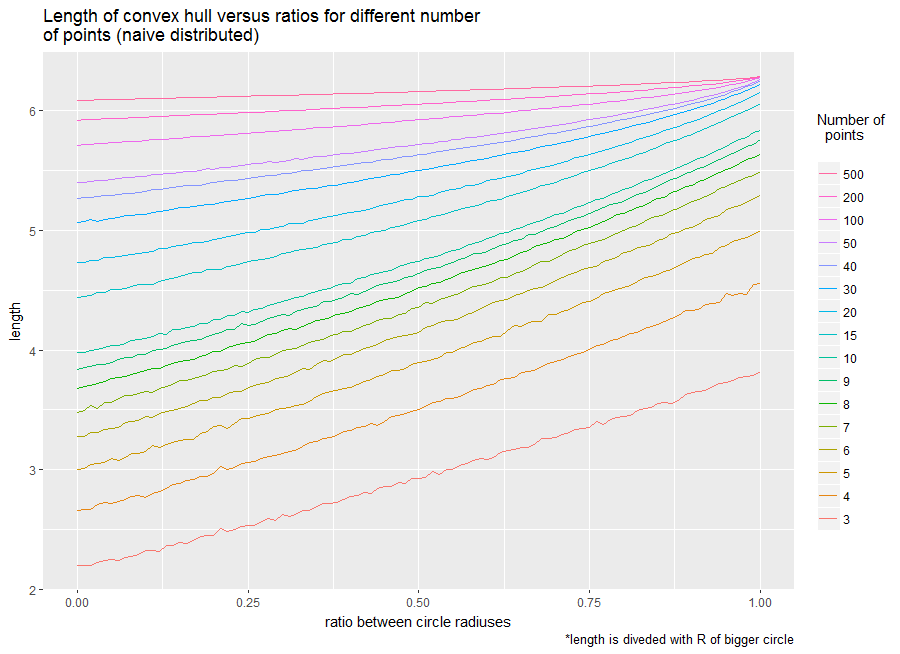
\includegraphics[width=0.55 \textwidth]{../graphs/graphs/length_naive.png}}
  \subfloat[With polar distribution]{
   \label{f:length2}
    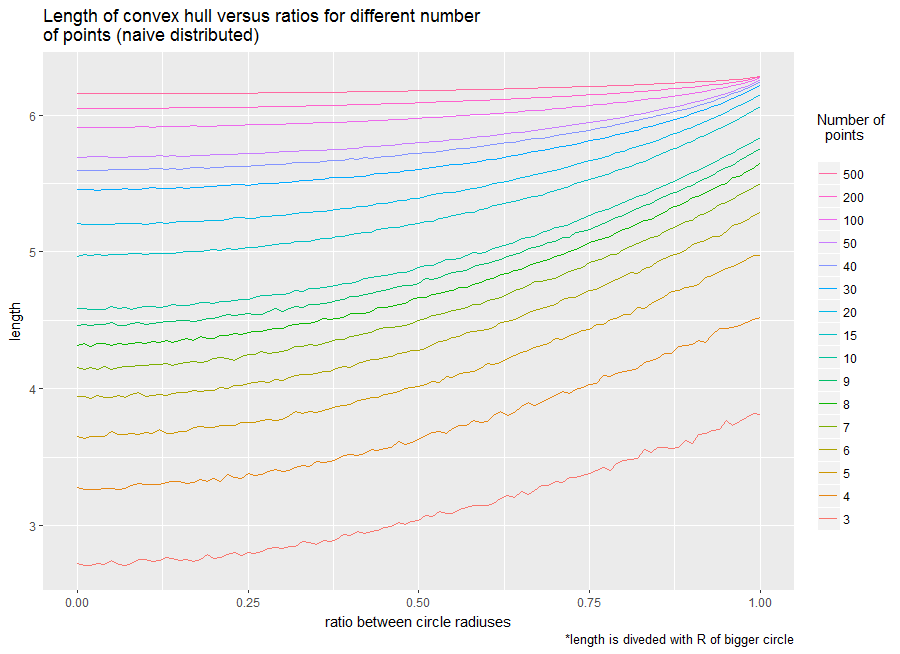
\includegraphics[width=0.55 \textwidth]{../graphs/graphs/length_polar.png}}
 \caption{Graphs with the results obtained when we calculate the convex hull length.}
 \label{f:results_length}
\end{figure} 

At first glance we can see, that the length of the convex hull increases proportionately to $n$ and $r$, as we suspected.

In order to reach a more precise conclusion and be able to analyse the data, we will superimpose the graphs.
\begin{figure}[H]
\centering
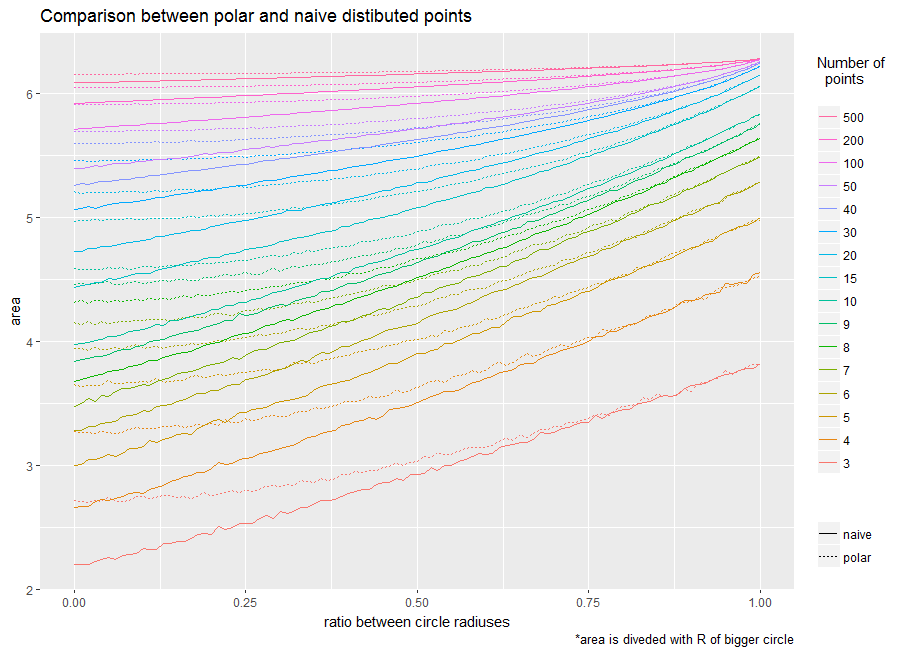
\includegraphics[scale=0.48]{../graphs/graphs/length_comparison.png}
\caption{Graph to compare the results of the length by the two distributions.}
\label{f:comparison_length}
\end{figure}

Now, we can see easily that our hypothesis about the length of the convex hull was correct. The length of the convex hull increases significantly with the number of points till a certain point and then only marginally with further increase. The length of the radius $r$ is also a significant factor in the length of the hull, especially at lower $n$. Length is a little more sensitive to $r$ than to $n$, especially at lower values, but not by a huge margin.\\
And also as expected the convex hulls, resulting from the data with polar distribution, have greater length. Also, as seen from Figure \ref{f:comparison_length}, points, generated with the polar method, have a less linear function in dependence of $r$ than those, generated with the other method.\\
When $r\to1$ and $n\to\inf$, we can see that the length approaches $2\pi$
\pagebreak 

\subsection{Area of the convex hull}


\begin{figure}[H]
 \centering
  \subfloat[With naive distribution.]{
   \label{f:area1}
    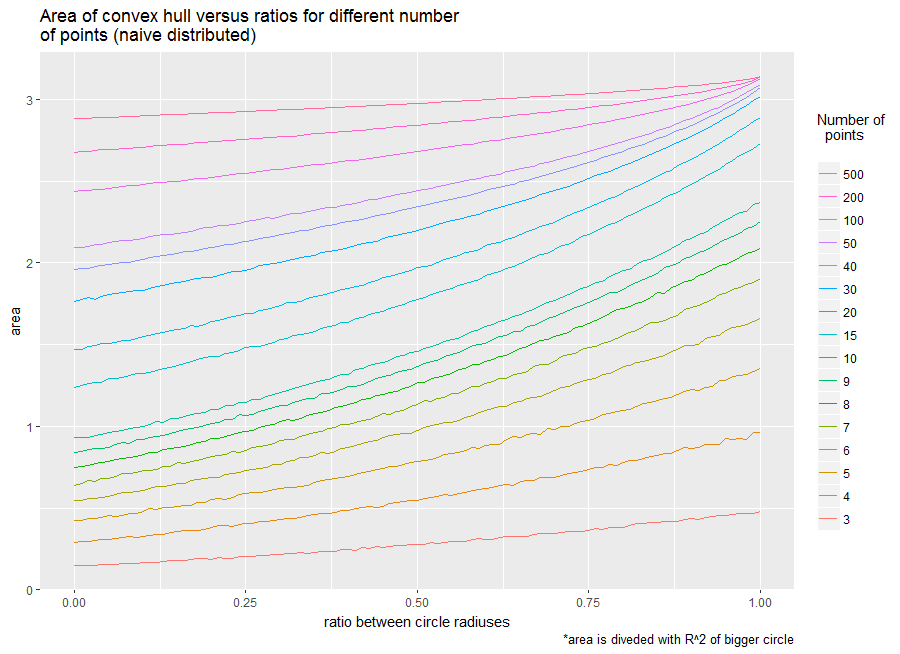
\includegraphics[width=0.55 \textwidth]{../graphs/graphs/area_naive.png}} 
  \subfloat[With polar distribution]{
   \label{f:area2}
    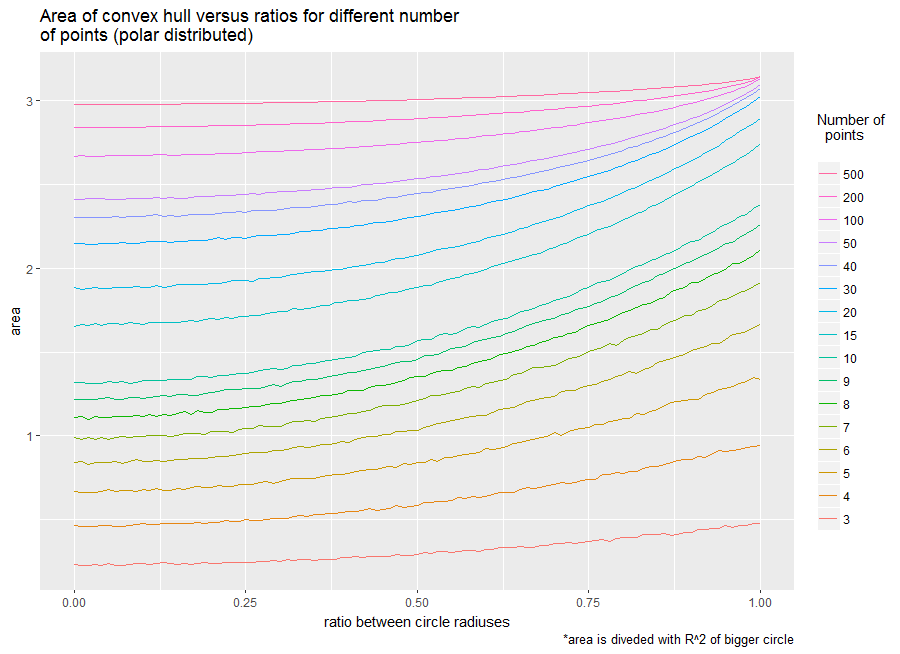
\includegraphics[width=0.55  \textwidth]{../graphs/graphs/area_polar.png}}
 \caption{Graphs with the results obtained when we calculate the convex hull area.}
 \label{f:results_area}
\end{figure}

When first looking at the graphs, we can see that the area increases, as expected, with $n$ and $r$.

\begin{figure}[H]
\centering
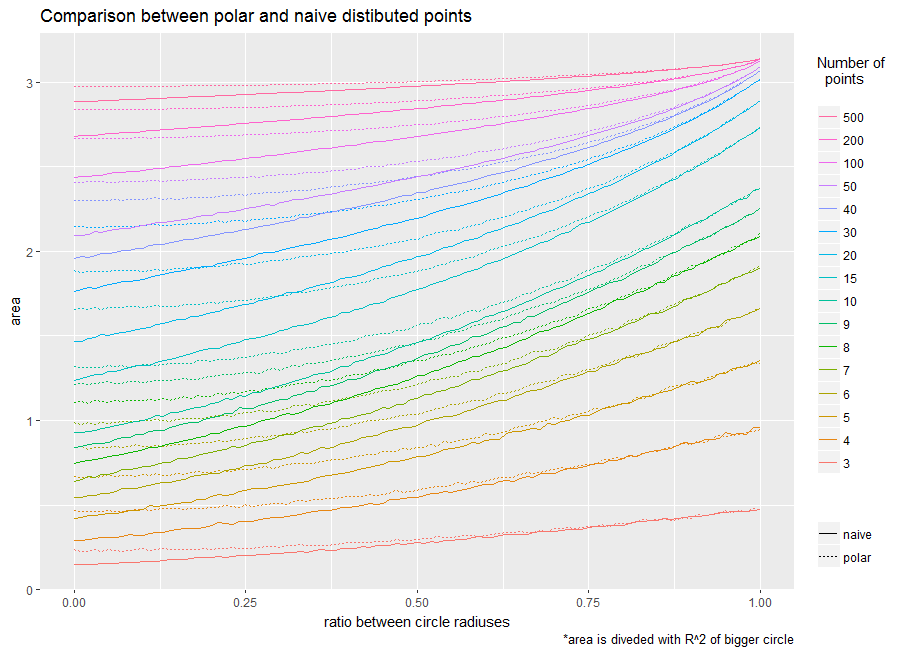
\includegraphics[scale=0.63]{../graphs/graphs/area_comparison.png}
\caption{Graph to compare the results of the area by the two distributions.}
\label{f:comparison_area}
\end{figure}

After superimposing (Figure \ref{f:comparison_area}), we can clearly see that the points, that were generated using the polar method, generate a convex hull with a larger area. Here the effects of $r$ and $n$ are similar. When $n$ is low, $r$ has less of an impact than when it is high. The biggest effect, as read from the plot, is when $n$ is about $10$. \\
When $n\to\inf$ and $r\to1$, the area converges to $\pi$, which is expected. The results for the area are also in line with our hypothesis. \pagebreak

\subsection{Probability of the convex hull contains the small circumference:}
\begin{figure}[H]
 \centering
  \subfloat[With naive distribution.]{
   \label{f:prob1}
    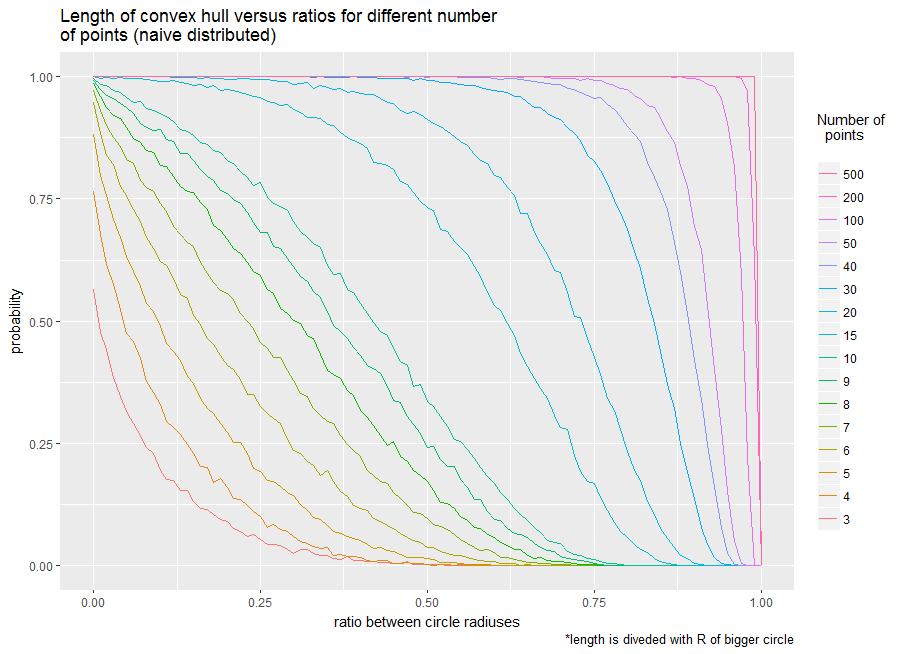
\includegraphics[width=0.55 \textwidth]{../graphs/graphs/probability_naive_new.png}} 
  \subfloat[With polar distribution.]{
   \label{f:prob2}
    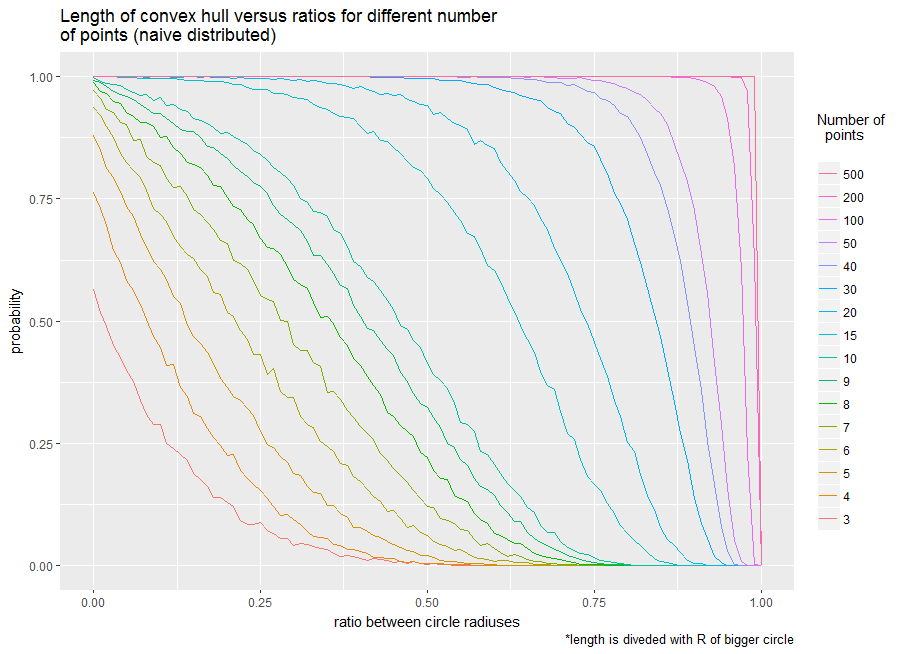
\includegraphics[width=0.55  \textwidth]{../graphs/graphs/probability_polar_new.png}}
 \caption{Graphs with the results obtained when we calculate the probability of the convex hull contains the small circumference $C'$.}
 \label{f:results_prob}
\end{figure}

We can see that the probability, that the convex hull includes the smaller circle ($C'$), increases with $n$ and decrease with $r$ in both cases, which is quite intuitive and expected.

Now we going to observe the comparison of both distributions
%hbtp
\begin{figure}[H]
\centering
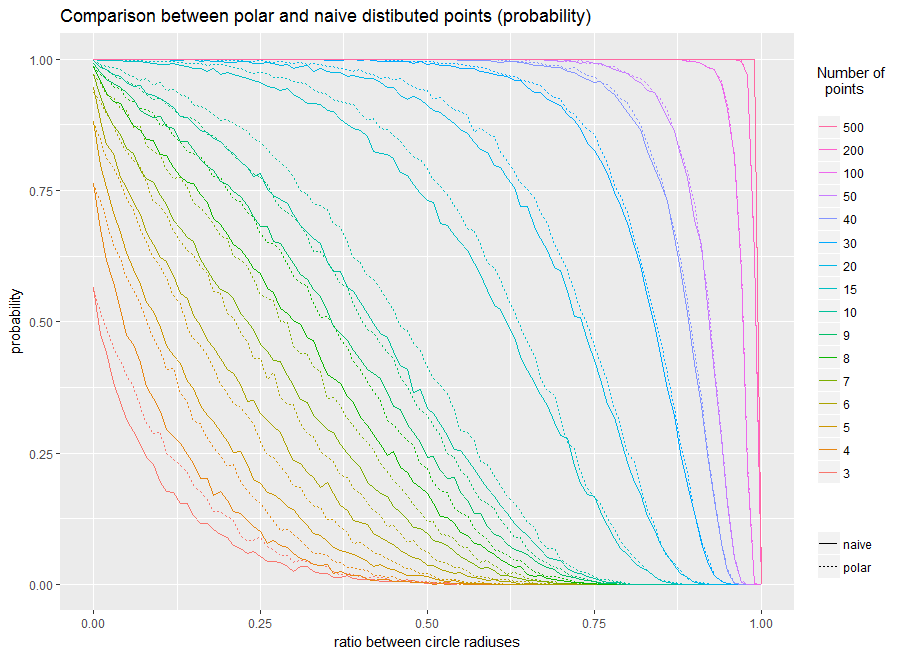
\includegraphics[scale=0.63]{../graphs/graphs/probability_comparison_new.png}
\caption{Graph to compare the results of the probability by the two distributions.}
\label{f:comparison_probability}
\end{figure}

The shape of both curves changes, when we use a different $n$. For a lesser $n$, the curve is convex, and when we increase it, it changes to a concave curve.. The change starts when $n$ is around $10$. This means that to this point, the probability is more responsive to $r$ and from this point onwards, the probability is less and less responsive to it. This happens, because with greater number of points comes a bigger probability, that the vertices will be near the edge, and won't be effected by a small increase of $r$.\\

With the same $r$, the probability of including the smaller circle is higher when the vertices were generated using the polar method. This makes sense, as those vertices are more spaced out, in contrast to those, generated using the naive method, which are biased to the middle.  \\
 
To finish and  complete the analysis, we have added two 3D-graphs with which the results are much better visualised globally.
\begin{figure}[H]
 \centering
  \subfloat[With naive distribution.]{
   \label{f:prob1}
    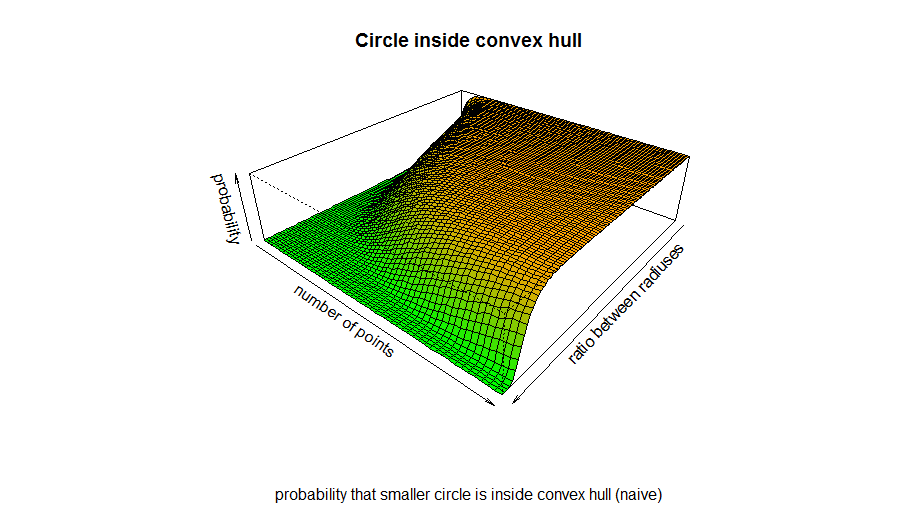
\includegraphics[width=0.53 \textwidth]{../graphs/graphs/3D_naive_new.png}}
  \subfloat[With polar distribution.]{
   \label{f:prob2}
    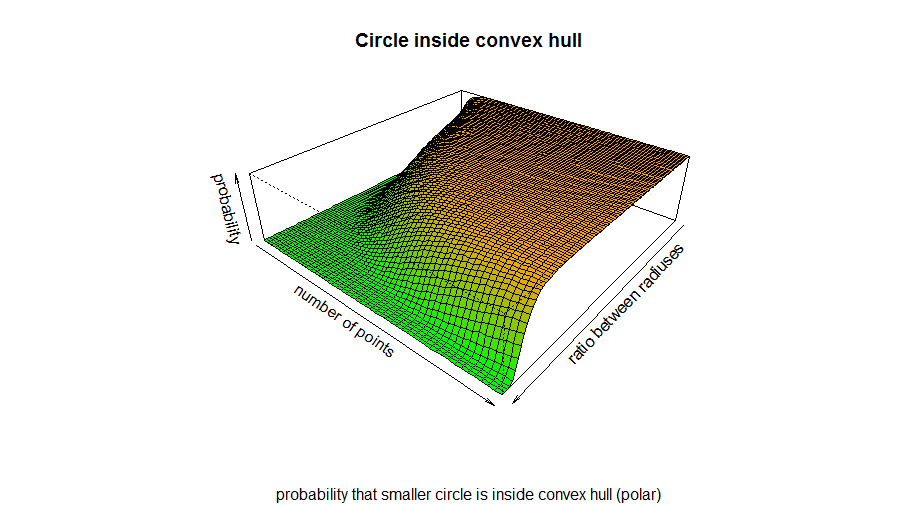
\includegraphics[width=0.53  \textwidth]{../graphs/graphs/3D_polar_new.png}}
 \caption{Graphs 3D with the results obtained}
 \label{f:results_prob}
\end{figure}

With this section we have finished analysing the results and comparing them to our hypothesis. It was, almost fully, correct. 

\section*{Bibliography}
\begin{enumerate}
\item Cormen, Thomas H.; Leiserson, Charles E.; Rivest, Ronald L.; Stein, Clifford (2001) [1990]. "33.3: Finding the convex hull". Introduction to Algorithms (2nd ed.). MIT Press and McGraw-Hill. pp. 955–956. ISBN 0-262-03293-7.

\item Jarvis, R. A. (1973). "On the identification of the convex hull of a finite set of points in the plane". Information Processing Letters. 2: 18–21. doi:10.1016/0020-0190(73)90020-3.
\end{enumerate}




\end{document}